\insertmeeting 
	{Bright Ideas, Great Solutions} 
	{10/22/22} 
	{Hagerty High School}
	{Jorge, Nathan, Ritam}
	{Images/RobotPics/robot.jpg}
	{1:30 - 3:30}
	
\hhscommittee{CAD}
\noindent\hfil\rule{\textwidth}{.4pt}\hfil
\subsubsection*{Goals}
\begin{itemize}
    \item Check design of prototype with mentor for any modifications or adjustments
    \item Get started on the design for the final drivetrain


\end{itemize} 

\noindent\hfil\rule{\textwidth}{.4pt}\hfil

\subsubsection*{Accomplishments}
At the start of today’s meeting, we talked to one of our mentors to review our prototype design and make sure that there was nothing wrong with it that may cause unforeseen problems in the future. Because the mentor we consulted has an engineering background (running the innovation lab and UCF, competing in the DARPA grand challenge, a self-driving car competition, and much more) we felt that there was no one better to give us advice on how to improve our design than him. After seeing our prototype, he had several suggestions. His first was to use bearings and shafts to make the steering knuckle turn smoother and last longer. This was already something we planned to do on the real design, but hadn’t implemented on the prototype for simplicity and ease of construction. His next suggestion, however, was less expected. He told us that on real cars and RC cars, the steering knuckle is taller, connecting to the chassis of the car at 2 points which were much farther away from each other than they were on our design (figure 1). Making the steering knuckles taller, not only will reduce the risk of snapping them off in a collision, but will hold the wheels more rigidly than in our prototype. His final suggestion, which built on his previous one, was to create a separate piece to hold the steering knuckle that would bolt onto the chassis instead of being incorporated into it as one piece. This would make the printer able to make the layer lines go in a different direction than the rest of the chassis, allowing us to strengthen the design and prevent it from splitting on a layer line. Additionally, if we wanted to create the part out of metal in the future, we wouldn’t have to re-print the whole drivetrain and could just replace that one part.

Taking these ideas into account we got into CAD and started designing the front part of our chassis. We started by fixing the issues our mentor had pointed out,  making the steering knuckle taller and creating a part separate from the rest of the chassis to hold it (figure 2) after making those parts, we started making the rest of the chassis, but soon encountered an issue. One problem we had seen but overlooked on the prototype was that the tie bar could hit the chassis, limiting the max steering angle. We wanted to aim for a max angle of 60 degrees, which was the amount the front wheel was limited to on the tricycle design we had tested with. Wanting to preserve this higher angle of steering which would allow us to turn sharper, we started thinking of ways to change the shape of the chassis or knuckle connection bracket to stop the tie bar from interfering with the steering angle. After trying several ideas, we decided to place the knuckle connection bracket at an angle, moving it out of the way of the tie bar. This worked, increasing our max turn angle from about 45 degrees to 66.92 degrees, more than our target! With that issue fixed, we connected the two sides in an assembly, making sure to add large ribs to maintain strength, finishing the basic shape of the front of the drivetrain (figure 3).


 

\begin{figure}[ht]
\centering
\begin{minipage}[b]{.48\textwidth}
  \centering
  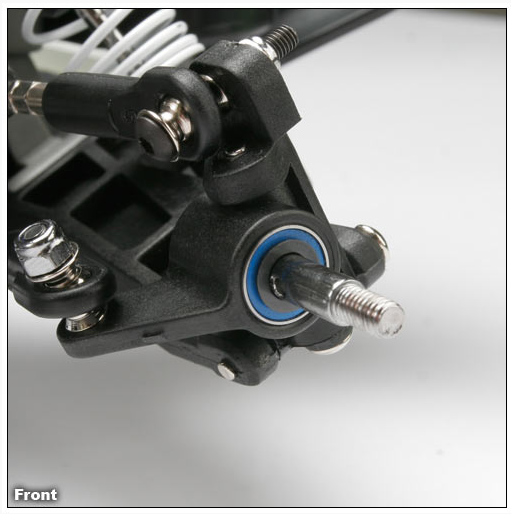
\includegraphics[width=0.95\textwidth]{Meetings/October/10-22-22/10-2-22_CAD_Figure1.PNG}
  \caption{Drive team on field}
  \label{fig:pic1}
\end{minipage}%
\hfill%
\begin{minipage}[b]{.48\textwidth}
  \centering
  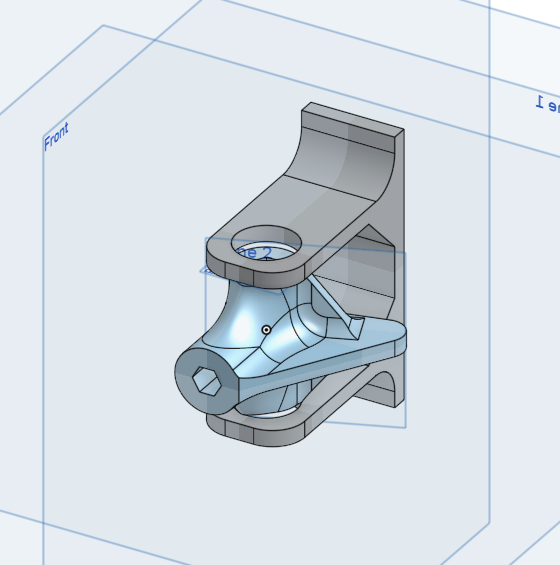
\includegraphics[width=0.95\textwidth]{Meetings/October/10-22-22/10-2-22_CAD_Figure2.PNG}
  \caption{Robot at first meet}
  \label{fig:pic2}
\end{minipage}
\end{figure}
\begin{figure}[ht]
\hfill%
\begin{minipage}[b]{.48\textwidth}
  \centering
  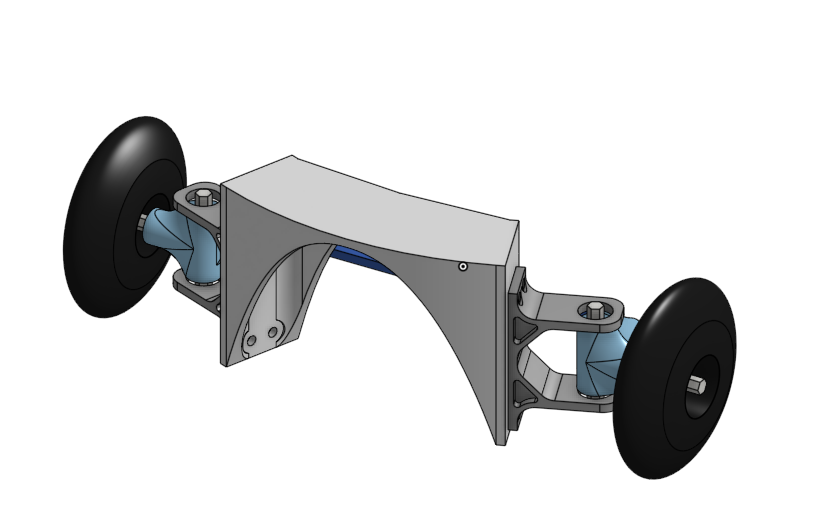
\includegraphics[width=0.95\textwidth]{Meetings/October/10-22-22/10-2-22_CAD_Figure3.PNG}
  \caption{Robot at first meet}
  \label{fig:pic2}
\end{minipage}
\end{figure}

\whatsnext{
\begin{itemize}
    \item Finish the back half of the drivetrain
    \item Modify old design to finish chassis


    
\end{itemize} 
}
